\input{../../university/.preambles/01-semester_work}
\input{../../university/.preambles/10-russian}
\input{../../university/.preambles/20-math}
\input{../../university/.preambles/30-physics}
\begin{document}
	
	Последнее обновление: %%%date%%%

	\emph{4.1:}\\

	Согласно Томпсоновской модели атом представляет собой непрерывно положительно 
	заряженный шар, внутри которого находятся электроны колеблющихся около своих
	положений равновесия.
	Пункт а: \\
		\[ E_1 = kr\frac{e}{R^3} \]
		\[ E_2 = k\frac{e^2}{r^2} \]
		\[ 
			E_\text{ион.} = \int^R_0 E_1 e dr + \int^\infty_R E_2 e dr = 
			\int^R_0 kr\frac{e^2}{R^3} + \int^\infty_R kr\frac{e^2}{r^2} =
			\frac{ke^2}{2R} + \frac{ke^2}{R} = \frac{3ke^2}{2R}
		\]
		\[
			R = \frac{3ke^2}{2E_\text{ион.}}
		\]
	Рассмотрим пункт б: \\
		\[ E_{внут.} = kr\frac{e}{R^3} \]
		\[ F = -e\cdot E = -kr\frac{e^2}{R^3} \]
	С учётом \( F = ma \) или \( F = m\ddot{r} \) получаем:
		\[ m\ddot{r} = -kr\frac{e^2}{R^3} \]
		\[ \ddot{r} + \frac{ke^2}{mR^3}r = 0 \]
	Обозначим \( \omega^2 = \cfrac{ke^2}{mR^3} \). \\

	\emph{4.2:}\\

	Так как \( \alpha \)-частица и ядро атома свинца положительные частицы, то
	энергия их взаимодействия будет иметь вид, представленный на рисунке:

	\begin{figure}[b!]
	    \center
	    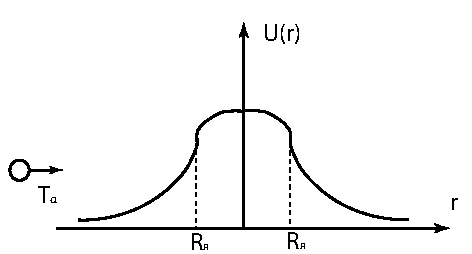
\includegraphics[width=0.47\textwidth]{4_2.pdf}
	\end{figure}

	Таким образом для приближения \( \alpha \)-частицы к ядру существует потенциальный
	барьер. Условие отражения \( \alpha \)-частиц от ядра атома свинца будет иметь вид:
		\[ T_\alpha \leq U_max \approx \frac{3}{2}\frac{q_1 q_2}{r_{min}} \]
	где \( q_1 = 2e \) -- заряд \( \alpha \)-частицы, \( q_2 = 82e \) -- заряд ядра свинца. \\
	Из формулы получим: \( r_{min} \approx R_\text{я} \approx 9.6\cdot10^{-10} \) см. \\
	Для более точного расчёта \( T = \cfrac{2ze^2}{r_{min}} \), где z = 82.\\

	\emph{4.4:}\\
		\[ p = \mu v_\text{отн} = \frac{m_2}{m1+m2}\cdot p_1 \]
		\[ p_1 = \sqrt{2mK} \]
		\[ \mu = \frac{m1\cdot m2}{m1+m2} \]
		\[ m1 = m;\quad m_2 = M \]
		\[ p = \frac{\sqrt{2mK}}{1+\cfrac{m}{M}} \]
		\[ K = \frac{p^2}{2\mu} = \frac{K}{1+\cfrac{m}{M}} \]

	\emph{4.6:}\\
	Прицельный параметр \( b \) можно найти из формулы:
		\[ tg\frac{\theta'}{2} = \frac{q_1 q_2}{2bT_1} \]
		\[ b = \frac{q_1 q_2}{2T_1}ctg\frac{\theta}{2} \]
	Так как \( \theta \) и \( T \) это параметры в Ц -- системе, 
	необходимо перейти в Л -- систему:
		\[ T_1 = \frac{m_2}{m_1 + m_2} = \frac{4}{5}T \]
	Следовательно
		\[ 
			b = \frac{2e^2\cdot 5}{2\cdot 4\cdot T}ctg{30^\circ} 
			\approx 2.4\cdot 10^{-11} \text{см} 
		\]

\end{document}